
%(BEGIN_QUESTION)
% Copyright 2006, Tony R. Kuphaldt, released under the Creative Commons Attribution License (v 1.0)
% This means you may do almost anything with this work of mine, so long as you give me proper credit

If we poke a hole at the bottom of a vessel containing an otherwise static column of liquid, we have an application for Bernoulli's equation at three different points in the system:

$$\includegraphics[width=15.5cm]{i00446x01.eps}$$

Note that point 1 has no velocity or pressure, but it does have elevation (height); point 2 has no velocity or elevation, but it does have pressure; and point 3 has no elevation or pressure, but it does have velocity.

Use Bernoulli's equation to write a new equation relating the elevation of point 1 with the pressure of point 2 and the velocity of point 3, and then solve for the velocity at point 3 in terms of the other two points' non-zero variables.

\vskip 10pt

\noindent
{\bf Bernoulli's equation:}

$$z_1 \rho g + {v_1^2 \rho \over 2} + P_1 = z_2 \rho g + {v_2^2 \rho \over 2} + P_2$$

\underbar{file i00446}
%(END_QUESTION)





%(BEGIN_ANSWER)

$$z_1 \rho g + {v_1^2 \rho \over 2} + P_1 = z_2 \rho g + {v_2^2 \rho \over 2} + P_2 = z_3 \rho g + {v_3^2 \rho \over 2} + P_3$$

$$z_1 \rho g + 0 + 0 = 0 + 0 + P_2 = 0 + {v_3^2 \rho \over 2} + 0$$

$$z_1 \rho g = P_2 = {v_3^2 \rho \over 2}$$

\vskip 10pt

$$v_3 = \sqrt{2 g z_1}$$

$$v_3 = \sqrt{2 P_2 \over \rho}$$

\vskip 10pt

The Pitot tube converts the outlet stream's velocity head ($v^2 \rho \over 2$) into a stagnation pressure head ($P$), then into an elevation head ($z \rho g$).

\vskip 10pt

Challenge question: explain why a {\it Pitot tube} placed in the path of the outlet stream generates a liquid column equal in height to $z_1$:

$$\includegraphics[width=15.5cm]{i00446x02.eps}$$

%(END_ANSWER)





%(BEGIN_NOTES)


%INDEX% Physics, dynamic fluids: Torricelli's theorem derived from Bernoulli's equation

%(END_NOTES)


